%!TEX root = notas_de_clase.tex

\section{Procesos gaussianos}


Como se vio en capítulos anteriores, el problema de regresión busca encontrar una función $y= f(x)$, dado un conjunto de pares de la forma $\mathcal{D}=\{(x_i, y_i)\}_{i=1}^N$. Dentro de los métodos vistos para resolver el problema de regresión, se vio el de regresión lineal, lineal en los parámetros y no lineales. Una característica en común que tienen estos métodos es que el proceso de entrenamiento consiste en encontrar un número fijo de parámetros, que minimicen cierta función objetivo, donde la cantidad de parámetros y la forma del modelo es parte del diseño. A este tipo de modelos se les llama \textit{modelos paramétricos}.\\

En contraste, se encuentran los modelos \textit{no paramétricos} los cuales no tienen un número fijo de parámetros, donde pueden llegar a ser en algunos casos infinito. Un ejemplo es el algoritmo de $k$-vecinos más cercanos (KNN), donde los puntos del conjunto de entrenamiento son usados para clasificar nuevas muestras. Otro ejemplo son las máquinas de soporte vectorial (SVM) donde al entrenar se obtienen los vectores de soporte.\\

Es importante hacer la distinción entre parámetros que se aprenden y los parámetros del modelo, muchas veces llamados hiperparámetros, donde estos últimos pueden ser fijos independiente si el método es paramétrico o no paramétrico. Esto se ve en el caso de SVM donde los parámetros serían los vectores de soporte, y los hiperparámetros serían el tipo de kernel, los parámetros de dicho kernel y los demás valores elegidos de antemano que definen el tipo de modelo.\\

En este capítulo introduciremos un método no paramétrico probabilístico de regresión no lineal, llamado procesos gaussianos ($\gp$). Este modelo en vez de encontrar un candidato único de la función a estimar, define una distribución sobre funciones $\mathbb{P}(f)$, donde $f$ es una función de un espacio de entrada $\mathcal{X}$ a los reales, $f: \mathcal{X} \rightarrow \mathbb{R}$. Esto tiene la virtud de permitir cuantificar la incertidumbre puntual que existe en la predicción de nuestro modelo, la cual servirá en forma de intervalos de confianza para la distribución gaussiana.\\

Partiremos definiendo un $\gp$ como una distribución a priori sobre funciones, y mostraremos que la densidad posterior se puede encontrar de forma exacta y que esta también es un $\gp$, conservando sus propiedades.\\

Es importante notar que si $\mathcal{X}$ tiene cardinalidad infinita (por ejemplo $\mathcal{X}=\mathbb{R}$), $f$ puede ser visto como un vector infinito dimensional. Como en la práctica no podemos trabajar con un vector infinito dimensional, dados $n$ puntos $\{ x_i\}_{i=1}^{n}  \subset \mathcal{X}$, podemos definirn el vector $n$-dimensional de valores de la función evaluada en dichos puntos $f(\mathbf{x})=(f(x_1), \ldots, f(x_n))^\top$.

\begin{definition}[proceso gaussiano]
	Un proceso gaussiano ($\gp$) es una colección de variables aleatorias, tal que para cualquier subconjunto finito de puntos, estos tienen una distribución conjuntamente gaussiana.
\end{definition}

Al aplicar esta definición a nuestro caso anterior, $\pr(f)$ será un $\gp$ y para cualquier conjunto finito $\{ x_i\}_{i=1}^{n}  \subset \mathcal{X}$, la distribución de $\pr(f(\mathbf{x}))$ es Gaussiana multivariada $f(\mathbf{x})=(f(x_1), \ldots, f(x_n))^\top$). En este caso las variables aleatorias representan el valor de la función $f(x_i)$ en la posición $x_i$.\\

Un $\gp$ queda completamente caracterizado por su función de media $m(\cdot)$ y función de covarianza $K(\cdot, \cdot)$, de esta forma para cualquier conjunto finito podemos encontrar la distribución. Definimos estas funciones como
\begin{align}
	m(x) & = \mathbb{E}\left\{f(x)\right\}\\
	K(x, x') & = \mathbb{E}\left\{\left(f(x) - m(x)\right) \left(f(x') - m(x') \right)\right\}
\end{align}

Y de esta forma podemos escribir el proceso como:

\begin{equation}
	f \sim \gp(m(\cdot), K(\cdot, \cdot))
\end{equation}

Donde para un conjunto finito tenemos que la marginal resulta de la forma:

\begin{equation}
	f(\x) \sim \mathcal{N}(m(\x), K(\x, \x))
\end{equation}

Hasta el momento hemos hablado del espacio de entrada $\mathcal{X}$ como genérico, un caso común es definir los $\gp$ sobre el tiempo ($\mathbb{R}^{+}$), es decir que los $x_i$ son instantes de tiempo. Es de notar que este no es el único caso, y se podría definir sobre un espacio más general, por ejemplo $\mathbb{R}^d$.\\

Otro punto a notar es que como estamos hablando de una colección (no necesariamente finita) de variables aleatorias, es necesario que se cumpla la propiedad de marginalización (o llamada consistencia\footnote{Para más detalles puede ver el teorema de consistencia de Kolmogorov}). Esta propiedad se refiere a que si un $\gp$ define una distribución multivariada para digamos dos variables $(y_1, y_2) \sim \mathcal{N}(\mu, \Sigma)$ entonces también debe definir $y_1 \sim \mathcal{N}(\mu_1, \Sigma_{11})$ donde $\mu_1$ es la componente respectiva del vector $\mu$ y $\Sigma_{11}$ la submatriz correspondiente de $\Sigma$. En otras palabras, el tomar un subconjunto más grande de puntos no cambia la distribución de un subconjunto más pequeño. Y podemos notar que esta condición se cumple si tomamos la función de covarianza definida anteriormente.

\subsection{Muestreo de un prior $\gp$}

Como fue mencionado, un $\gp$ define un \textit{prior} sobre funciones, por lo que, antes de ver ningún dato se podría obtener una muestra de este proceso dado una función de media y covarianza. Un supuesto común es asumir la función de media $m(\cdot)=0$ por lo que solo nos queda definir una función de covarianza o kernel, un ejemplo de kernel es el \textit{Exponencial Cuadrático} (Square Exponential), también conocido como RBF (Radial Basis function) o Kernel Gaussiano (en general se evita este nombre porque este kernel no tiene relación con la distribución de los datos).

\begin{equation}
	K_{SE}(x, x') = \sigma^2 \exp\left( - \frac{\left( x- x'\right)^2}{2\ell^2} \right)
\end{equation}

Donde en este caso los parámetros son interpretables (y como veremos más adelante pueden ser aprendidos a través de un conjunto de entrenamiento) donde $\sigma^2$ es la varianza de la función, notar que esta es la diagonal de la matriz covarianza. El parámetro $\ell$ es conocido como el \textit{lenghtscale} que determina que tan lejos tiene influencia un punto sobre otro, donde en general un punto no tendrá influencia más allá de $\ell$ unidades alrededor.\\

Como sabemos, las funciones definidas por el $\gp$ son vectores infinito dimensionales, por lo que no podemos muestrear de toda la función, pero tomando una cantidad suficiente de puntos podemos graficar muestras de un $\gp$ dada una función de covarianza. Tomando un $\gp$ con media cero ($m(\cdot)=0$) y kernel SE, muestras del proceso para distintos valores de $\ell$ obtenemos la Fig.\ref{fig:gp_1}, donde el área sombreada corresponde al intervalo de confianza del $95\%$. Se puede ver que el parámetro $\ell$ controla que tan erráticas son las funciones, donde a medida que va a aumentando las muestras se vuelven funciones más suaves.

\begin{figure}[H]
	\centering
	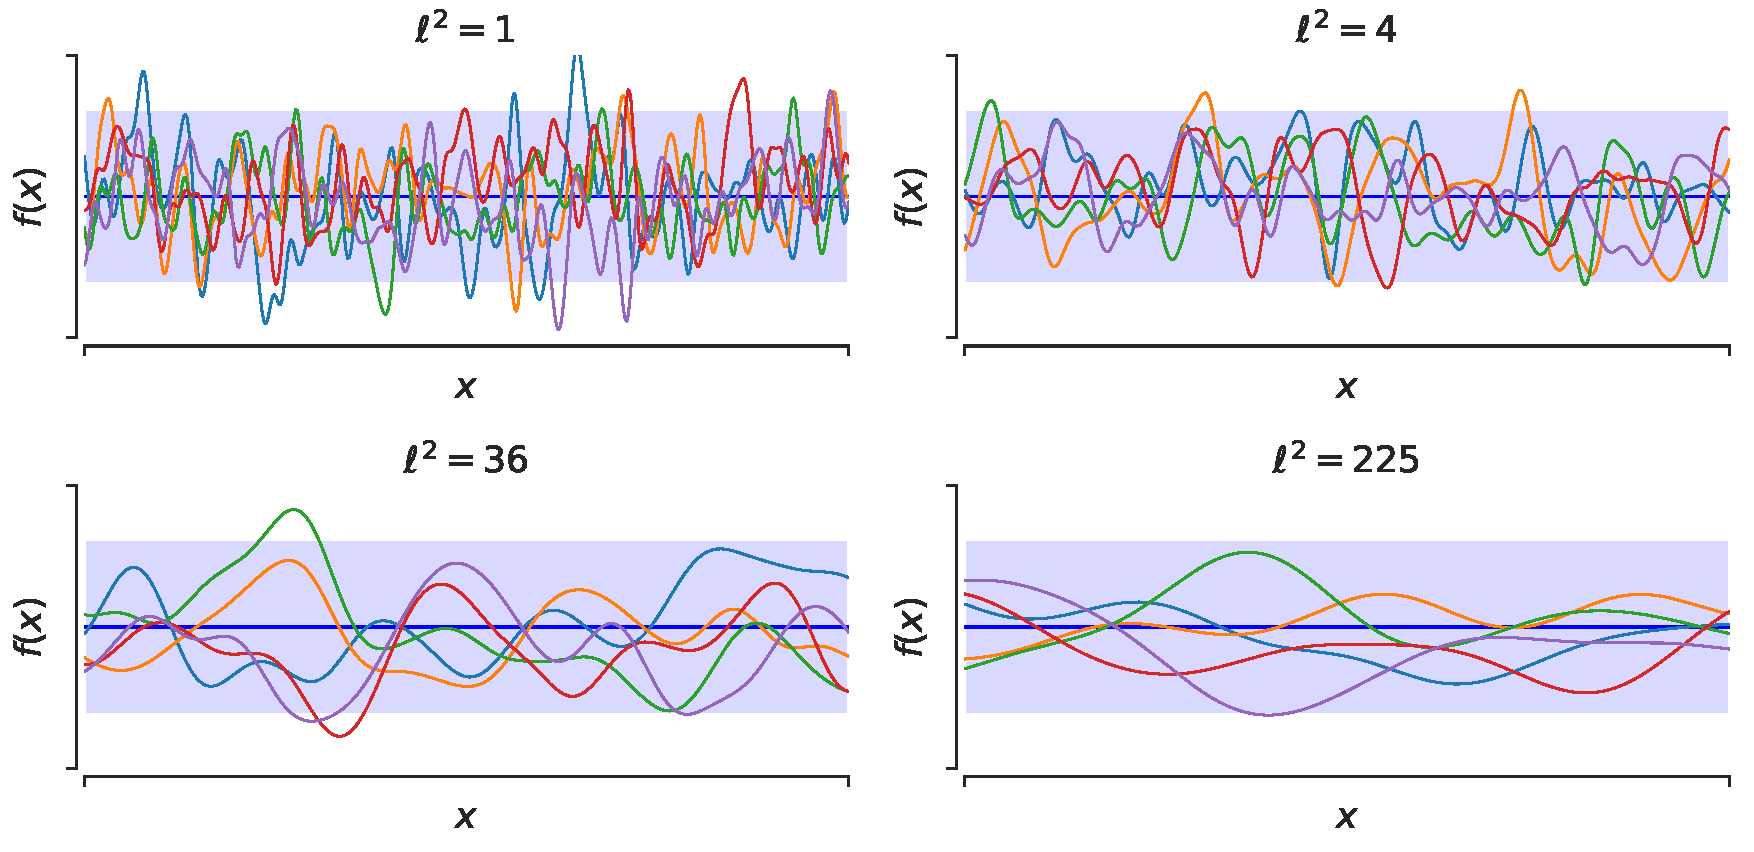
\includegraphics[width=0.9\textwidth]{img/cap8_prior_muestras}
	\caption{Muestras de un prior $\gp$ con kernel SE, para distintos \textit{lenghtscales} ($\ell$) y función media $m(\cdot)=0$, la parte sombreada corresponde al intervalo de confianza del $95\%$. Se puede ver que a mayor $\ell$ las funciones se van volviendo más suaves.}
	\label{fig:gp_1}
\end{figure}

\subsection{Incorporando información}

Ahora que ya podemos muestrear de nuestro prior, nos interesaría incorporar las observaciones que tenemos de la función a nuestro modelo. Para esto, se pueden considerar dos casos: observaciones con ruido y observaciones sin ruidos (o deterministas).

\subsubsection{Evaluación sin ruido}

 En el caso de las observaciones sin ruido, tenemos observaciones de la forma $\{(x_i, f(x_i))\}_{i=1}^{n}$, donde tenemos el valor real de nuestra función en los puntos $[x_1, \ldots, x_n]=X$. Luego, tenemos el par de entradas y observaciones $(X,f(X))$. Digamos que queremos realizar una predicción en el conjunto $X_*$ de $n_*$ puntos, luego la distribución conjunta es de la forma:
\begin{align}
	\begin{bmatrix} f(X) \\ f(X_*)  \end{bmatrix}
	\sim \mathcal{N} \left(
	\begin{bmatrix} m(X) \\ m(X_*)  \end{bmatrix}, 
	\begin{bmatrix}
		K(X, X) & K(X, X_*) \\ K(X_*, X) & K(X_*, X_*)
	\end{bmatrix}
	 \right)
\end{align}

Donde la submatriz $K(X, X_*)$ es de $n \times n_*$, $K(X, X)$ de $n \times n$ y así respectivamente para cada submatriz. Dada las observaciones y una función de covarianza, podemos evaluar la verosimilitud, que también es gaussiana, lo que nos lleva a un punto clave de los processos gaussianos:

\begin{lemma}
	Dado un prior $\gp$ sobre $f(\cdot)$ y una verosimilitud Gaussiana, la posterior sobre $f(\cdot)$ es también un $\gp$. Además, se puede condicionar sobre las observaciones $(X, f(X))$ para obtener

\begin{equation}
	f(X_*)|f(X), X  \sim \mathcal{N}(m_{X_*|X}, \Sigma_{X_*|X}) \label{eq:gp_post}
\end{equation}

Donde la media y covarianza son:
\begin{align}
	m_{X_*|X} & = m(X_*) + K(X_*, X)K^{-1}(X, X) (f(X) - m(X))\\
	 \Sigma_{X_*|X} & = K(X_*, X_*) - K(X_*, X)K^{-1}(X, X) K(X, X_*)
\end{align}
\end{lemma}

Ahora, dado un conjunto de observaciones y dada una función de covarianza, podemos obtener la densidad posterior. Para mostrar esto tomemos el caso de hacer regresión para una función conocida, para la cual tenemos observaciones sin ruido muestreadas no uniformemente, con estas observaciones queremos encontrar la función real de las que provienen; para esto usamos un prior $\gp$ con función media nula y kernel SE (por el momento tendrá parámetros fijos), nos damos un rango donde queremos hacer predicción y condicionamos en las observaciones usando la Ec.(\ref{eq:gp_post}). En este caso las observaciones corresponden al 15$\%$ de los puntos generados por nuestra función sintética.\\

Esto se muestra en la Fig.\ref{fig:gp_2}, donde podemos ver que la media de la posterior pasa por las observaciones sin incertidumbre asociada, es decir que para estos puntos se tiene una posterior degenerada pues no hay varianza. Se puede ver que a medida que la predicción se aleja de las observaciones el intervalo de confianza (al que lo podemos asociar con incertidumbre del modelo) va creciendo.

\begin{figure}[H]
	\centering
	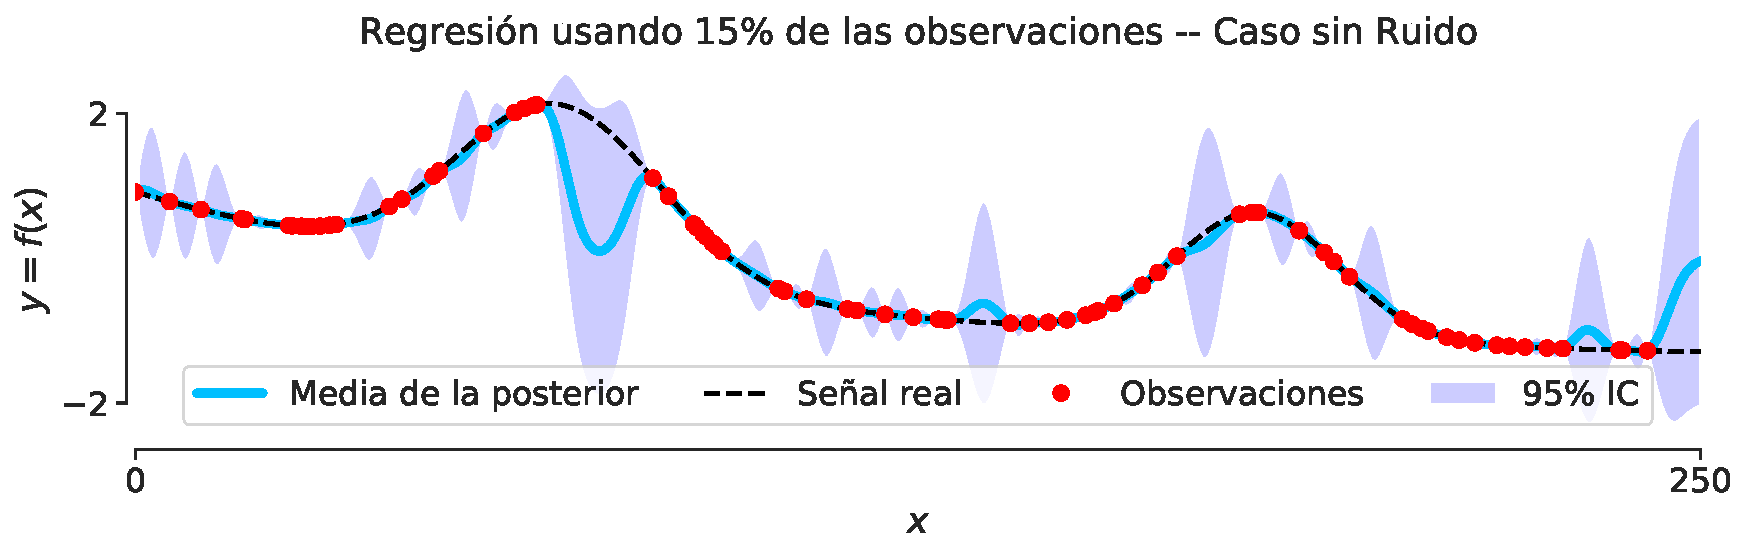
\includegraphics[width=0.9\textwidth]{img/cap8_posterior_no_ruido}
	\caption{Regresión con $\gp$ para señal sintetica usando el 15$\%$ de los datos muestreados de forma no uniforme, utilizand un $\gp$ de media nula y kernel SE.} 
	\label{fig:gp_2}
\end{figure}

\subsubsection{Evaluación con ruido}

En aplicaciones reales el caso de tener observaciones sin ruido es poco habitual, por lo que si queremos incorporar la incertidumbre real debemos tomar en cuenta errores de medición en nuestro modelo. Tomemos el caso de tener observaciones contaminadas con ruido i.i.d (independientes idénticamente distribuidas) donde las observaciones serán de la forma $y_i = f(x_i) + \eta$ donde $\eta \sim \mathcal{N}(0, \sigma_n^2)$, por lo que ahora nuestro conjunto de observaciones es de la forma $(X,Y)$ donde $Y=f(X) + \eta$.

Lo que en nuestro modelo equivale a agregar un término a la función de covarianza

\begin{equation}
	cov(Y) = K(X, X) + \sigma_n^2\eye
\end{equation}

Donde si tenemos el mismo caso anterior, observaciones $(X,Y)$ y queremos evaluar en $X_*$, la conjunta queda
\begin{align}
	\begin{bmatrix} Y \\ f(X_*)  \end{bmatrix}
	\sim \mathcal{N} \left(
	\begin{bmatrix} m(X) \\ m(X_*)  \end{bmatrix}, 
	\begin{bmatrix}
		K(X,X) + \sigma_n^2 \eye & K(X, X_*) \\ K(X_*,X) & K(X_*,X_*)
	\end{bmatrix}
	 \right)
\end{align}

Notemos que el termino de ruido solo es agregado al subbloque correspondiente a las observaciones, no se agrega el termino en los otros subbloques pues buscamos hacer una predicción de la función latente $f(\cdot)$ y no una versión ruidosa de esta.
Igual que en el caso sin ruido, podemos condicionar esta conjunta a las observaciones y obtenemos el siguiente resultado:

\begin{lemma}
	Para una evaluación con ruido se tiene que
	
	\begin{equation}
		f(X_*)|Y, X  \sim \mathcal{N}(m_{X_*|X}, \Sigma_{X_*|X})\label{eq:gp_posterior}
	\end{equation}
	Donde la media y covarianza son:
	\begin{align}
		m_{X_*|X} & = m(X_*) + K(X_*, X) [K(X, X) + \sigma_n^2 \eye]^{-1} (Y - m(X))\\
	 \Sigma_{X_*|X} & = K(X_*, X_*) - K(X_*, X) [K(X, X) + \sigma_n^2 \eye]^{-1} K(X, X_*)
	\end{align}
\end{lemma}

Si tomamos el mismo ejemplo anterior, pero añadimos el ruido al modelo, obtenemos la predicción de la Fig.\ref{fig:gp_3}. En este caso podemos ver que la media de la posterior no necesariamente coincide su valor con el de la observación, pues se toma en cuenta la incertidumbre en las observaciones mismas, también se ve que no se obtienen soluciones degeneradas incluso en zonas donde hay observaciones aglomeradas.


\begin{figure}[H]
	\centering
	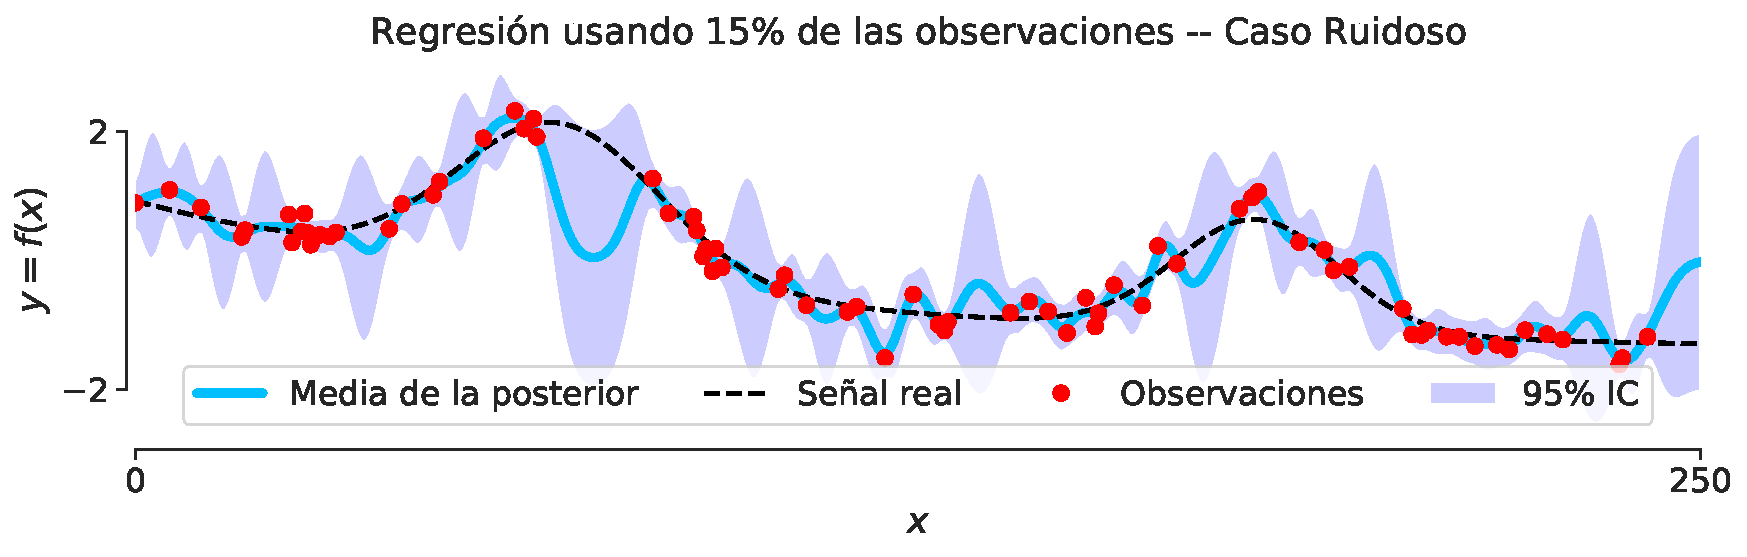
\includegraphics[width=0.9\textwidth]{img/cap8_posterior_ruido}
	\caption{Regresión con $\gp$ para señal sintetica usando el 15$\%$ de los datos muestreados de forma no uniforme y contaminados con ruido Gaussiano, utilizando un $\gp$ de media nula y kernel SE.}
	\label{fig:gp_3}
\end{figure}

\subsection{Entrenamiento y optimización de un $\gp$}

hasta el momento nos hemos dado la función de covarianza y sus parámetros, por lo que aún no hemos hecho realizado el \textit{aprendizaje} de nuestro $\gp$, que es lo que haremos a continuación.

\subsubsection{¿Qué es entrenar un $\gp$?}

Vimos que dada una función de covarianza podemos representar el proceso, y podemos encontrar analíticamente la densidad posterior de nuestra función $f(\cdot)$ condicionando a las observaciones. Pero la forma que tendrá la posterior y la función fuera de las observaciones dependerá fuertemente en nuestra función kernel escogida, en este sentido, para un kernel dado nos gustaría encontrar los parámetros de este que mejor representen nuestra función a estimar.\\

Nos referiremos a entrenar u optimizar un $\gp$ cuando queremos obtener los hyperparámetros, es decir los parámetros del kernel (los denotamos $\theta$) y la varianza del ruido (la denotamos $\sigma_n^2$) si es que aplica.

Para esto nos gustaría poder comparar funciones de covarianza, o mejor aún un funcional que podamos optimizar, afortunadamente podemos usar la \textit{verosimilitud marginal}, obtenida marginalizando sobre la función $f(\cdot)$, donde dado un conjunto de entrenamiento $(X, Y)= \{(x_i, y_i)\}_{i=1}^{n}$, esta dada por

\begin{align}
	\pr(Y|X, \theta, \sigma) & = \int \pr(Y|f, X, \theta, \sigma_n) p(f|X,\theta, \sigma) df \\
	& = \frac{1}{\left( 2\pi |\mathbf{K}_y|\right)^{\frac{n}{2}}} 
	\exp \left(
	-\frac{1}{2} (Y - \mathbf{m})^T \mathbf{K}_y^{-1} (Y - \mathbf{m})
	\right)
\end{align}

Donde $\mathbf{m}=m(X)$ y $\mathbf{K}_y=K_{\theta}(X,X) + \sigma_n^2 \eye$, la matriz de covarianza dados los parámetros $\theta$ agregando el término de la diagonal correspondiente al ruido. De la misma forma que lo hacemos con otros modelos probabilísticos, en vez de maximizar la verosimilitud, en conveniente minimizar la log-verosimilitud negativa (NLL) dada por la expresión:

\begin{align}
	NLL & = -\log \pr(Y|X, \theta, \sigma_n) \\
	NLL & = \underbrace{ \color{black}{\frac{1}{2}\log|\mathbf{K_y}|} }_
	    {\text{\parbox{2cm}{\centering Penalización\\[-4pt] por\\[-4pt] complejidad}}}
	    + \underbrace{ \color{black}{\frac{1}{2}(Y - \mathbf{m})^T \mathbf{K}_y^{-1} (Y - \mathbf{m}) }}_
	    {\text{\parbox{4cm}{\centering Data fit (Única parte que depende de $Y$)}}}
	    + \underbrace{ \color{black}{\frac{n}{2} \log2\pi}}_
	    {\text{\parbox{2cm}{\centering Constante de normalización}}}\label{eq:gp_nll}
\end{align}

De izquierda a derecha, el primer término tiene el rol de penalizar por la complejidad del modelo, y vemos que depende solo del kernel y las entradas; el segundo término cuantifica que tan bien se ajusta el modelo a los datos, y es la única componente que depende de las observaciones $Y$ (ruidosas) de la función, el último término es una constante de normalización.\\


\begin{figure}[H]
	\centering
	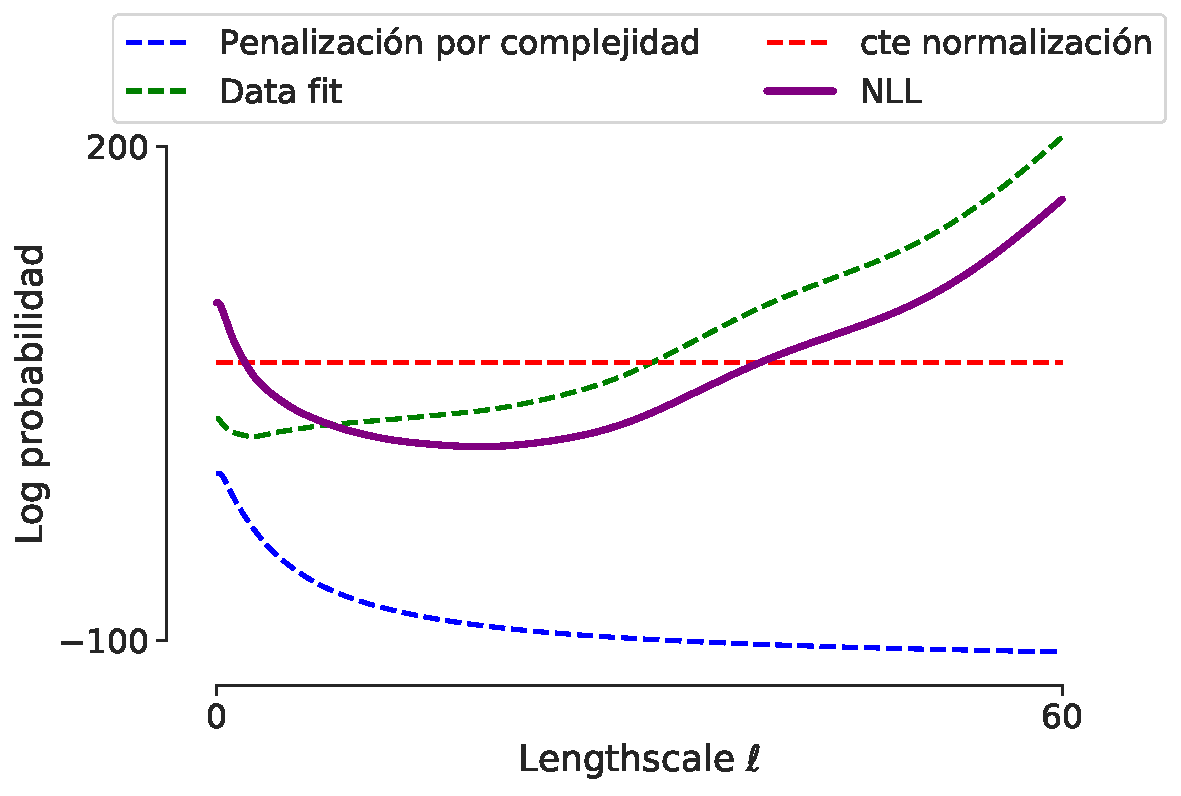
\includegraphics[width=0.5\textwidth]{img/cap8_nll_partes}
	\caption{Log verosimilitud marginal negativa (NLL) en función del \textit{lengthscale} ($\ell$) para señal sintetica, se mantienen constantes los otros parámetros del $\gp$.}\label{fig:gp_4}
	\label{fig:nll_por partes}
\end{figure}

Siguiendo con los ejemplos anteriores, para el mismo conjunto de observaciones ruidosas, se calculan las tres componentes de la $NLL$, utilizando un kernel SE, para este caso, se dejan fijo tanto la varianza de la señal como la varianza del ruido y se varia el \textit{lengthscale} $\ell$ del kernel, en la Fig.\ref{fig:gp_4}.

Al ir variando $\ell$ se ve que la penalización por complejidad va disminuyendo, pues a mayor $\ell$ menos complejas son las funciones (recordar Fig.\ref{fig:gp_1}, a mayor $\ell$ más suaves y regulares las muestras), también vemos que la componente del ajuste de datos comienza a decaer y luego se mantiene en incremento, pues a mayor \textit{lengthscale} el modelo se vuelve menos flexible, por lo que no es capaz de ajustarse de manera correcta a los datos. De esta forma, el proceso de entrenamiento dará preferencia a funciones que se ajusten bien a los datos sin ser tan complejas, ahora viendo el valor total del NLL vemos que este alcanza su mínimo en $\ell$ en el rango de $[10-30]$.\\


Ya tenemos una noción de que es entrenar un $\gp$, queremos minimizar la $NLL$ (Ec.(\ref{eq:gp_nll})) y encontrar los parámetros del kernel y del ruido (si aplica). Ahora discutiremos formas de optimizar este funcional.

\subsubsection{¿Cómo se entrena un \gp?}

Como contamos con una expresión cerrada para la NLL, podemos utilizar métodos clásicos de optimización, una opción es calcular el gradiente de esta función objetivo y aplicar algún método basado en gradiente, como L-BFGS; otra es utilizar el método de Powell que no requiere que la función sea diferenciable, por lo que no utiliza gradiente.\\


Siguiendo ejemplos anteriores, usando la misma señal sintética y las mismas observaciones ruidosas de la Fig.\ref{fig:gp_3}, ahora optimizamos nuestro $\gp$ utilizando L-BFGS, lo que nos entrega como resultado el mostrado en la Tabla.\ref{tab:gp_1} donde comparamos los parámetros del $\gp$ sin entrenar usado en la Fig.\ref{fig:gp_3}, podemos ver que no difiere mucho en cuanto a las varianzas, pues como es una señal sintética poseíamos control sobre la varianza del ruido, el valor obtenido luego de optimizar es cercano al valor real (0.2), vemos que el \textit{lengthscale} óptimo es concordante con lo analizado en la Fig.\ref{fig:gp_4}.

Por último, podemos ver la predicción usando este $\gp$ optimizado en la Fig.\ref{fig:gp_5} donde vemos que se tiene una del proceso más concordante con la función real, esto se ve especialmente en la zona con pocas observaciones, entre 50 y 100 para $x$, donde el $\gp$ sin entrenar presentaba mucha incertidumbre en esa zona, en cuanto ahora se tiene un intervalo de confianza más bien limitado pues la señal no era muy compleja.

\begin{table}[H]
\centering
\begin{tabular}{lcccc}
 & $\sigma_{\text{ruido}}$ & $\ell$ & $\sigma_{\text{señal}}$ & NLL\\ \hline
Sin entrenar & 0.2 & 3.1622 & 1 & $\mathbf{55.3538}$\\
Entrenado & 0.2067 & 18.7267 & 0.9956 & $\mathbf{17.6945}$\\
\end{tabular}
\caption{Resultado optimización $\gp$ y comparación con los parámetros sin entrenar.}
\label{tab:gp_1}
\end{table}


\begin{figure}[H]
	\centering
	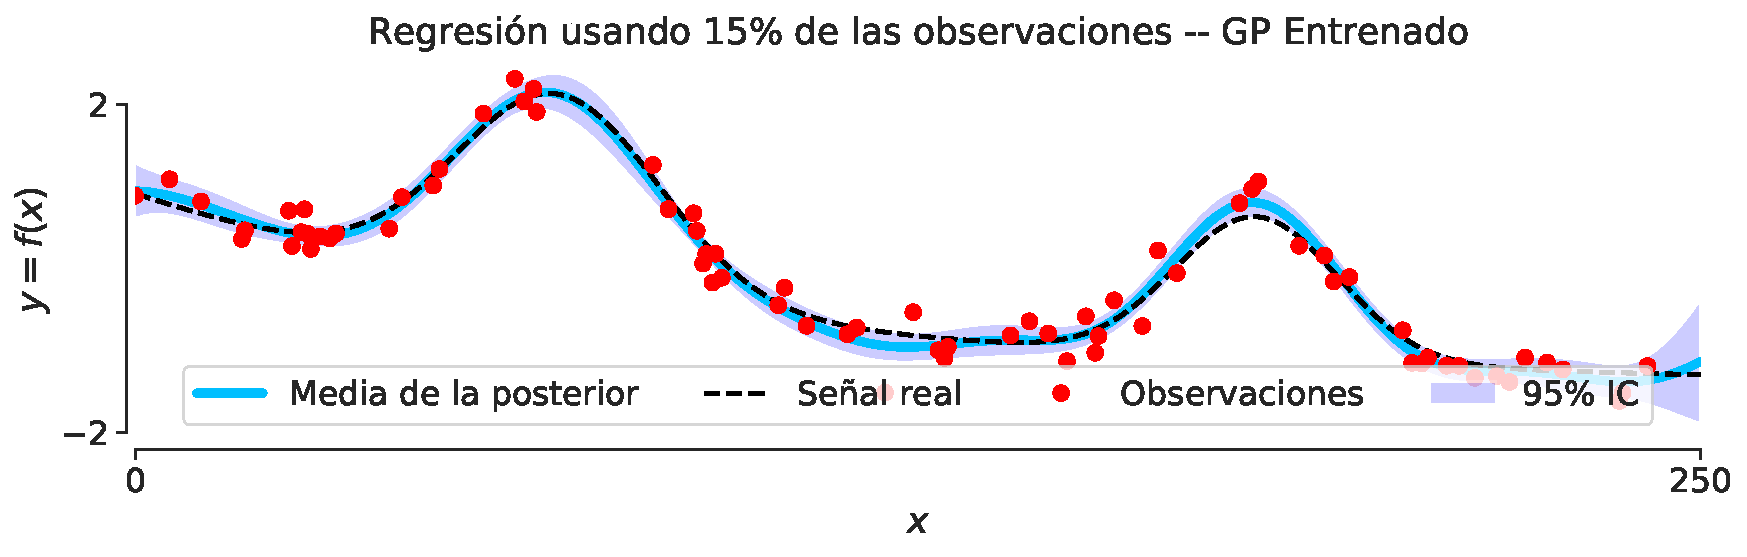
\includegraphics[width=0.9\textwidth]{img/cap8_entrenado}
	\caption{Regresión con $\gp$ para señal sintetica usando el 15$\%$ de los datos muestreados de forma no uniforme y contaminados con ruido Gaussiano, utilizando un $\gp$ de media nula y kernel SE; Modelo optimizado utilizando L-BFGS.}
	\label{fig:gp_5}
\end{figure}

La desventaja de utilizar métodos tradicionales de optimización es que estos entregan una solución puntual (en el sentido de un valor para cada parámetro, el $\gp$ sigue siendo una distribución sobre funciones), en distintas aplicaciones puede que un valor fijo de parámetros no represente de manera idónea el proceso latente a estudiar. Una opción sería computar la densidad posterior de los parámetros del kernel condicionado a las observaciones. Lamentablemente en la mayoría de los casos no existe una expresión cerrada para esta posterior, por lo que debemos recurrir a métodos de \textit{inferencia aproximada} como Markov Chain Monte Carlo (MCMC) o Inferencia Variacional.




% \subsubsection{Métricas de evaluación}
% ---pendiente---

\subsubsection{Complejidad computacional}

Es importante reconocer una de las principales desventajas de utilizar un $\gp$ cuando se cuenta con una gran cantidad de datos, esto es, su costo computacional.
Recordando, cuando queremos entrenar nuestro $\gp$ vamos a minimizar la log verosimilitud marginal negativa (NLL), mostrada en la Ec.(\ref{eq:gp_nll}), donde al observar en segundo término vemos que es la operación más costosa siendo $\mathcal{O}(n^3)$ con respecto al número de puntos de entrenamiento $n$. Hay que tomar en cuenta que la evaluación de la NLL se debe hacer en cada iteración del método de optimización elegido.

En cuanto a la evaluación, esta está dada por la Ec.(\ref{eq:gp_posterior}), donde en este caso vemos que es de orden cuadrático $\mathcal{O}(n^2)$ con respecto al número de puntos de test. Es de notar que esta vez no tomamos en cuenta la inversa de la matriz de Gram del conjunto de entrenamiento, pues puede ser precalculada y ser usada para múltiples conjuntos de test.\\

Lo anterior mencionado limita la cantidad de problemas que se pueden abordar usando estos procesos, sin embargo existen formas de obtener aproximaciones que siguen manteniendo la estructura y deseables propiedades de los $\gp$ a un menor costo computacional, estos reducen el orden de $\mathcal{O}(n^3)$ a $\mathcal{O}(nm^2)$ en entrenamiento y $\mathcal{O}(m^2)$ en test, con $m<n$. Un ejemplo de estos son los \textit{Sparse Gaussian Processes} que utilizan una aproximación de rango bajo para la matriz de covarianza, utilizando \textit{pseudo-inputs} en vez el conjunto de entrenamiento completo.


\subsection{Funciones de covarianza (kernels)}

Una función de covarianza es una función de dos argumentos donde cualquier matriz que se obtiene como resultado en la evaluación de un conjunto de puntos (la llamaremos matriz de Gram) es semidefinida positiva.

Hasta el momento solo hemos utilizado un tipo de función de covarianza, el llamado kernel \textit{Squared Exponential} (SE), conocido también como kernel RBF, dado por la Ec.(\ref{eq:gp_kernel_se}). En esta sección mostraremos distintos tipos de funciones de covarianza y los distintos tipos de funciones que generan.

\begin{equation}\label{eq:gp_kernel_se}
	K_{SE}(x, x') = \sigma^2 \exp\left( - \frac{\left( x- x'\right)^2}{2\ell^2} \right)
\end{equation}

Es importante denotar tipos de familias de funciones de covarianza, si la función solo depende de la diferencia, es decir $k(x, x')=k(x-x')$ se le llamará \textit{kernel estacionario}, más aún, si depende solo de la norma de la diferencia $k(x, x')=k(|x-x'|)$ se le llamará \textit{kernel isométrico}, un ejemplo de esto es el kernel SE.\\

Es de notar que kernels estacionarios hacen que la covarianza entre puntos sea invariante a traslaciones en el espacio de entradas. Una noción importante es que un kernel puede ser visto como una medida de similaridad entre puntos, y en el caso de kernels estacionarios, mientras más cercanos estén dos puntos más símiles serán.

\subsubsection{Rational Quadratic (RQ)}

Este kernel viene dado por la Ec.(\ref{eq:gp_kernel_rq}), este puede ser interpretado como una suma infinita de kernels SE con distintos \textit{lenghtscale}, donde $\alpha$ es un parámetro de variación de escala, notar que cuando $\alpha \rightarrow \infty$ el kernel tiende a uno SE. En la Fig.\ref{fig:gp_6} se muestra el kernel RQ, a la izquierda se ve el valor de la covarianza en función de la diferencia de los argumentos $x-x'$, a la derecha se muestran diferentes muestras de funciones con este kernel.
 
\begin{equation}\label{eq:gp_kernel_rq}
	K_{RQ}(x, x') = \sigma^2 \left(1 + \frac{\left( x- x'\right)^2}{2\alpha\ell^2 } \right)^{-\alpha}
\end{equation}


\begin{figure}[H]
	\centering
	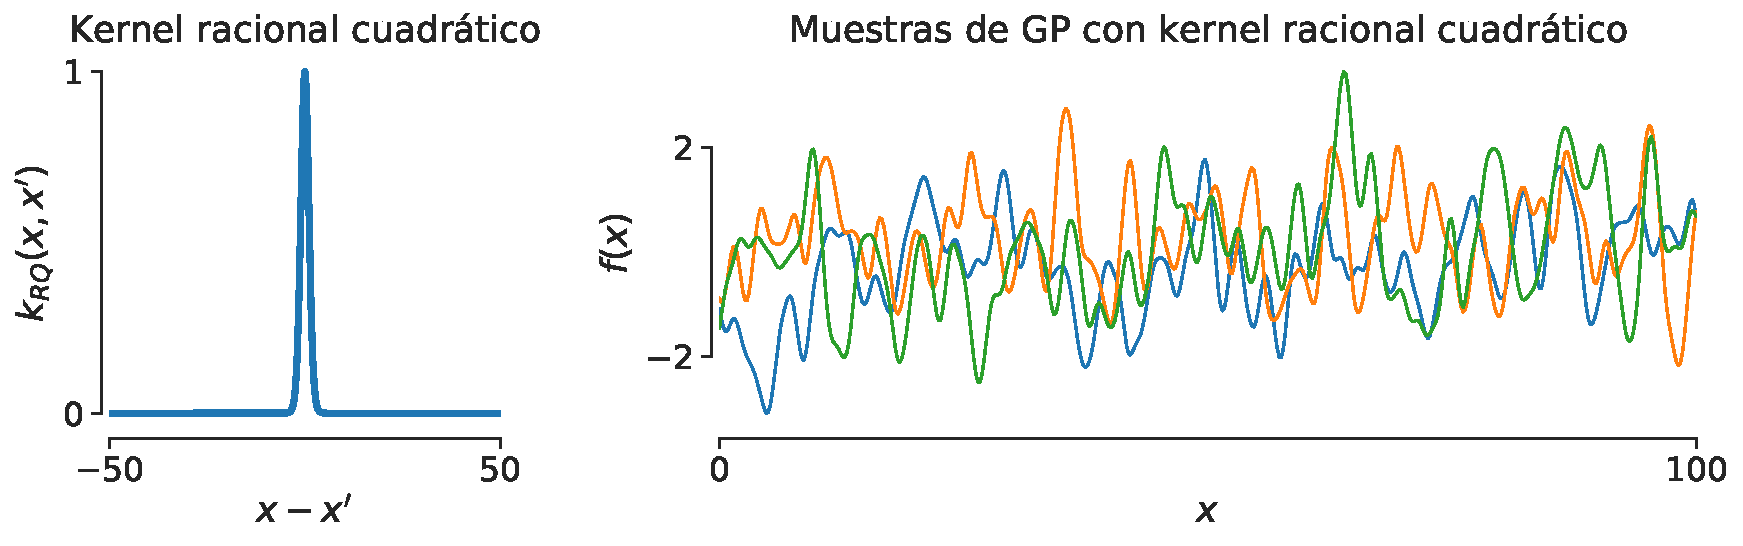
\includegraphics[width=0.9\textwidth]{img/cap8_muestras_RQ}
	\caption{Kernel \textit{Rational Quadratic}, en la izquierda se muestra la covarianza en función de su argumento $\tau=x-x'$, a la derecha de un $\gp$ usando un kernel RQ.}
	\label{fig:gp_6}
\end{figure}

\subsubsection{Kernel periódico}

Como su nombre lo indica, este kernel, dado por la Ec.(\ref{eq:gp_kernel_p}), permite modelar funciones periódicas, donde el parámetro $p$ controla el periodo de la función. Una extensión de este el kernel localmente periódico, dado por la Ec.(\ref{eq:gp_kernel_lp}) que es un kernel SE ponderado por uno periódico, este da la libertad de tener funciones con una estructura periódica local.


\begin{equation}\label{eq:gp_kernel_p}
	K_{P}(x, x') = \sigma^2 \exp\left(-\frac{2\sin^2\left(\pi |x- x'| / p \right)}{\ell^2 } \right)
\end{equation}

\begin{equation}\label{eq:gp_kernel_lp}
	K_{LP}(x, x') = \sigma^2  \exp\left(-\frac{\left(x- x' \right)^2}{2\ell^2 } \right) \exp\left(-\frac{2\sin^2\left(\pi |x- x'| / p \right)}{\ell^2 } \right)
\end{equation}

En la Fig.\ref{fig:gp_7} se muestra el kernel periódico, a la izquierda se ve el valor de la covarianza en función de la diferencia de los argumentos $x-x'$, a la derecha se muestran diferentes muestras de funciones con este kernel.

\begin{figure}[H]
	\centering
	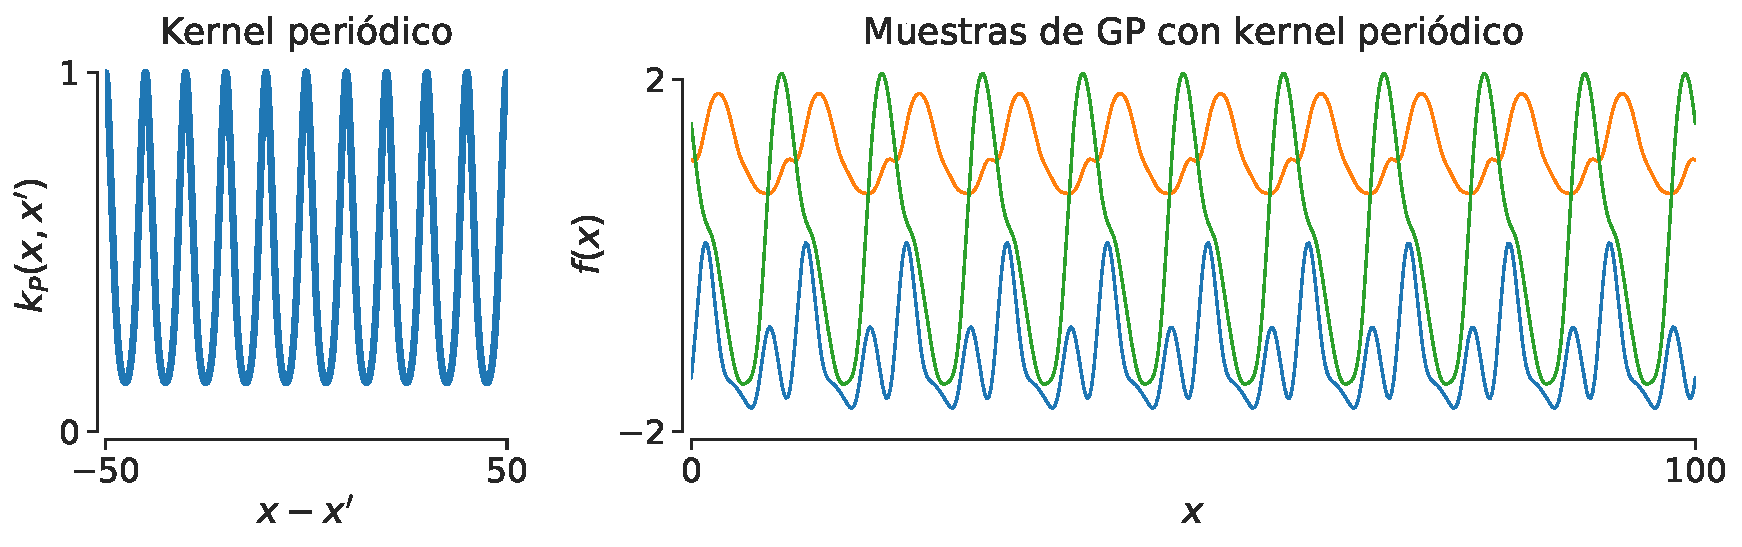
\includegraphics[width=0.9\textwidth]{img/cap8_muestras_P.pdf}
	\caption{Kernel periódico, en la izquierda se muestra la covarianza en función de su argumento $\tau=x-x'$, a la derecha de un $\gp$ usando un kernel periódico.}
	\label{fig:gp_7}
\end{figure}

\subsubsection{Operaciones con kernels}
A la hora de diseñar un $\gp$ y elegir una función de covarianza, no se está completamente limitado a kernels conocidos, sino que también se pueden combinar para obtener distintas funciones de covarianza y representar mejor el proceso.

Tanto la suma y multiplicación de kernels da como resultado un kernel válido que puede ser utilizado, también la exponencial de un kernel es también es un kernel, es decir $\exp(k_1(\cdot, \cdot))$ con $k_1$ un kernel válido.

\subsubsection{Representación espectral}
Un teorema importante para las funciones de covarianza en procesos débilmente estaicionarios es el teorema de Wiener–Khinchin, el cual dice que si para un proceso débilmente estacionario existe una función de covarianza $k(\tau)$ finita y definida para cualquier $\tau=x-x'$, entonces existe una función $S(\xi)$ tal que:

\begin{equation}\label{eq:gp_spectral}
	k(\tau) = \int S(\xi)e^{2\pi i \xi \cdot \tau} d\xi, \quad S(\xi)=\int k(\tau)e^{-2\pi i \xi \cdot \tau} d\tau
\end{equation}

Donde $i$ es la unidad imaginaria. $S(\xi)$ es conocida como la densidad espectral de potencia (PSD), en otras palabras, la función de covarianza $k(\tau)$ y la PSD $S(\xi)$ son duales de Fourier el uno del otro. Esto es extremadamente útil a la hora de diseñar funciones de covarianza pues este puede ser llevado a cavo en el dominio de la frecuencia y luego llevado a una función de covarianza usando la transformada inversa de Fourier.

\subsection{Extensiones para un $\gp$}
A continuación veremos un número de extensiones que se le pueden hacer a un $\gp$ para abordar distintos tipos de problemas.

\subsubsection{$\gp$ de clasificación}

\begin{wrapfigure}{r}{0.35\textwidth}
\centering
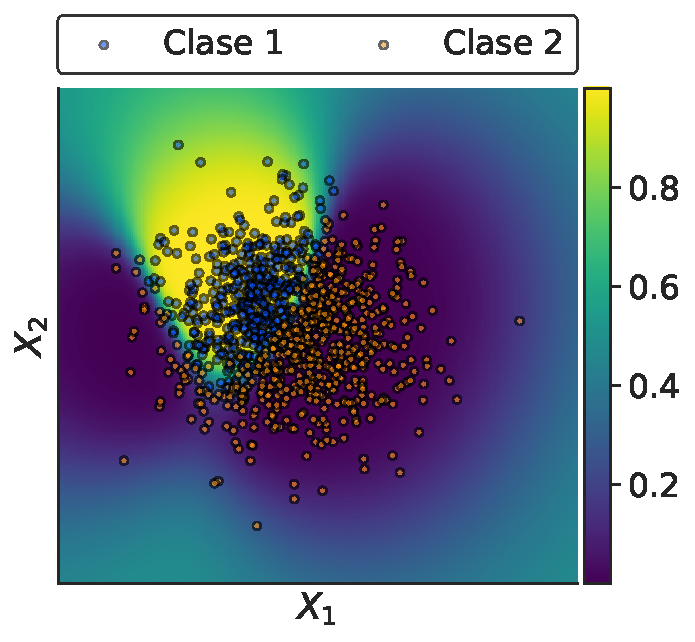
\includegraphics[width=0.3\textwidth]{img/cap8_classificacion}
\caption{$\gp$ de clasificación utilizando datos sintéticos. Este clasificador entrega una densidad de probabilidad en vez de una sola función de decisión.}\label{fig:gp_8}
\end{wrapfigure} 

Hasta el momento hemos visto como usar un $\gp$ para regresión, pero este también puede usado para clasificación, para esto simplemente ``pasamos'' nuestro $\gp$ por una función logística, para así obtener un prior sobre $\sigma\left(f(x)\right)$ donde $\sigma$ es la función logística. Sin embargo esto trae consigo un problema, pues ahora la distribución posterior a las observaciones no se tiene de forma analítica como para el caso de regresión, esto lleva a que tengamos que recurrir a métodos aproximado de inferencia. Una solución simple es utilizar la aproximación de Laplace, pero si se quieren aproximaciones más fidedignas métodos más complejos pueden ser usados como \textit{Expectation Maximization} y métodos MCMC. En la Fig.\ref{fig:gp_8} se muestra un ejemplo con datos sintéticos, a diferencia de la mayoría de los clasificadores vistos, este entrega naturalmente una densidad de probabilidad para la función de decisión.\\

\subsubsection{Selección automática de relevancia (ARD) (\textit{Selección automática de features})}
Un $\gp$ define una densidad de probabilidad sobre funciones, donde estas funciones son del tipo $f: \mathbb{R}^D \rightarrow \mathbb{R}$, con $D$ es finito, este es nuestra dimensión de entrada o ``características''. Haciendo un pequeño cambio en nuestra función kernel podemos hacer que esta automáticamente seleccione las entradas más relevantes con el problema, es decir realice una selección de características automática.\\

Si tomamos el kernel de la Ec.(\ref{eq:gp_ard}) vemos que es una multiplicación de kernels SE, donde se tiene un \textit{lenghtscale} por cada entrada $\ell_d$, sabemos que mientras más grande es este $\ell_d$ menos flexible será el $\gp$ respecto a cambios en ese eje, haciendo que las funciones del proceso dependan cada vez menos de la componente $d$ a medida que $\ell_d \rightarrow \infty$. De esta forma se puede controlar de forma automática la relevancia de cada eje del conjunto de entrada, pues los parámetros del kernel se obtienen en el entrenamiento. De esta forma estamos optimizando también en que grado afecta cada variable en nuestra predicción.

\begin{equation}\label{eq:gp_ard}
	k(x, x') = \sigma^2 \exp\left( -\sum_{d=1}^{D} \frac{(x_d - x_d')^2}{2\ell_d^2}\right)
\end{equation}


\subsubsection{Multi output $\gp$}
Hasta el momento solo hemos hablado de $\gp$ cuando nuestro proceso es solo una dimensión de salida. Se pueden extender los procesos Gaussianos a funciones de más de una salida o canal, donde ahora la función de covarianza $k(x, x')$ no entrega un escalar sino una matriz definida positiva, donde la diagonal corresponde a la covarianza del canal o autocovarianza y los elementos fuera de la diagonal corresponden a las covarianzas cruzadas o cross-covarianza. Este tipo de procesos Gaussianos aumentan considerablemente de complejidad al diseñar funciones de covarianza.\\ 

Dado un número $m$ de canales, se tendrán $m$ funciones de autocovarianza y ahora $m(m-1)/2$ funciones de covarianza y $k(x, x')$ será una matriz de $m\times m$. El desafio está en diseñar o escoger estas funciones de tal forma que para cualquier par de puntos $x$, $x'$ la matriz $k(x, x')$ sea definida positiva.

Una opción simple es asumir que los canales son independientes entre sí, lo que equivale a entrenar independientemente $m$ procesos Gaussianos, uno para cada canal, esto facilita el diseño de las funciones de covarianza pero hace que se pierdan relaciones entre los canales.
 

\subsection{Diferentes interpretaciones de un $\gp$}

\subsubsection{De regresión lineal a $\gp$}

Partiendo de la regresión lineal donde el modelo es:

\begin{equation}
	y_i = w X_i + \epsilon_i
\end{equation}

Donde $\epsilon_i \sim \mathcal{N}(0, \sigma_n^2)$, luego podíamos extender este modelo usando $M$ funciones base $\phi_m$ y obtener:

\begin{equation}
	y_i = \sum_{m=1}^{M} w_m \phi(x_i) + \epsilon_i
\end{equation}

El paso siguiente es la regresión Bayesiana en base de funciones, donde agregamos un prior sobre los pesos $w_m \sim \mathcal{N}(0, \lambda_m^2)$, donde si obtenemos la covarianza de este proceso y marginalizamos por los pesos $w_m$ obtenemos:

\begin{equation}
	Cov(x, x') = k(x, x') = \sum_{m=1}^{M} \lambda_m^2 \phi_m(x)^T\phi_m(x') + \delta_{x, x'} \sigma_n^2
\end{equation}

Donde $\delta_{x, x'}$ el delta de Kronecker. Si nos damos cuenta esto define un $\gp$ con la función covarianza con un número finito de funciones bases. En general los $\gp$ corresponderán a covarianzas con infinitas funciones bases, como veremos a continuación.\\

Tomando un modelo sin ruido, con un número $M$ de funciones base $\phi_m$, donde sobre los pesos se define un prior i.i.d $w_m \sim \mathcal{N}(0, \sigma^2)$, tenemos:

\begin{equation}
	f(x) =  \sum_{m=1}^{M} w_m \phi(x)
\end{equation}
Y tomando $\phi=\exp(-\frac{1}{2\ell^2}(x- c_i)^2)$ donde $c_i$ son los centros de estas bases, y luego haciendo tender el número de funciones base $M$ a infinito tenemos que la covarianza es:

\begin{align}
	\mathbb{E}\left\{f(x) f(x')\right\} & = \sigma^2\sum_{m=1}^{M}  \phi_m(x)\phi_m(x') && \text{tomando } M\rightarrow \infty\\
	\mathbb{E}\left\{f(x) f(x')\right\} & \rightarrow \sigma^2 \int e^{-\frac{1}{2\ell^2}(x- c)^2} e^{-\frac{1}{2\ell^2}(x'- c)^2} dc \\
	& = \sigma^2 \sqrt{\pi\ell^2} e^{-\frac{1}{4\ell^2}(x- x')^2}\\
	& = k_{SE}(x, x')
\end{align}

Donde vemos que efectivamente el kernel SE es una función de covarianza para una composición infinita de funciones base.

\subsubsection{Nota sobre RKHS}
Dado un conjunto de entrenamiento $(X, Y) = \{x_i, y_i \}_{i=1}^{n}$ condicionando el proceso solo a una muestra de test $X_*=x_*$ y asumiendo una función media nula, de la Ec.(\ref{eq:gp_post}) para un $\gp$ la posterior de la media está dada por:

\begin{equation}
	\bar{f}(x_*) = m_{x_*|X} = k(X, x_*) (k(X, X) + \sigma_n \eye)^{-1} Y
\end{equation}

Y tomamos el vector $\bm{\alpha} = \left(k(X, X) + \sigma_n \eye \right)^{-1} Y$ obtenemos la expresión:

\begin{equation}
	\bar{f}(x_*) = \sum_{i=1}^{n} \alpha_i k(x_i, x_*)
\end{equation}

Donde, a pesar de que el proceso esta descrito por (posiblemente infinita) funciones base, aún así es la suma de finitos términos, cada uno centrado en un punto de entrenamiento, esto es debido al teorema del representante de los Espacios de Hilbert de Kernel Reproductor (RKHS). La intuición detrás de esto es que incluso si el $\gp$ induce una distribución conjunta sobre todos los $y = f(x)$, una para cada $x$ en el dominio, al hacer predicciones en el punto $x_*$ solo nos interesa la distribución $(n+1)$-dimensional definida por los puntos de entrenamiento más este punto de test.
